%-----------------------------------------------------------------
%	CONCLUSIONS
%	!TEX root = ./../main.tex
%-----------------------------------------------------------------
\section{Results and Discussion}\label{sec:results}

\subsection{Parameter control}\label{sec:parameter-control}

As \textcite{Michalewicz2000} put it, typically, only one parameter is tuned at a time, which may result in some less-than-optimal choices because parameters interact in complex ways. The simultaneous tuning of more parameters, however, leads to an enormous amount of experimentation. The technical drawbacks of parameter tuning based on experimentation are:
\begin{itemize}
	\item The parameters are not independent, but trying all possible combinations is practically impossible.
	\item The process of parameter tuning is time consuming, even if parameters are optimised one at a time.
	\item The results are often disappointing, even when a significant expenditure of time is made.
\end{itemize}

Following this reasoning, and keeping in mind we want to find the balance between exploitation and exploration, we will try to find the right parameters for our $N$ Queens Problem. Ideally, our aim is to find a general value for the tournament size $\tau$ and the mutation probability $p$, independent problem size $N$; in contrast, the initial population size should depend on $N$.

Therefore, we have to find the minimum of a function $f$ such that:
\begin{align}
	\mqty{
		f:& \mathbb{N} \times \mathbb{R} \times \mathbb{N} & \to & \mathbb{N} \\
		& (\tau, p, \inline{POPULATION}) & \mapsto & \inline{iter}.
	}
\end{align}

Obviously, this function $f$ is an abstract one with an unpredictable behaviour. So, one wonders how to find the best parameters for a given $N$. \textcite{Michalewicz2000} thoroughly discuss previous literature on the topic of parameter control, only to conclude that even if one assumes for a moment that there is a perfect configuration, finding it is really a hopeless task.

\bigskip
To ease the hard task of finding somehow optimal parameters, we will stick with $\tau = 2$ (the most popular setting in Genetic Algorithms), and try to tune our algorithm playing with other parameters of the algorithm. This means our algorithm will probably lean slightly towards an exploratory approach, as we will not have a tunable variable to make the algorithm more exploitatory.

Our analysis will consist on playing with the following settings:
\begin{itemize}
	\item Mutation: $p \in [0.005, 0.01]$ with a step of $\Delta p = 0.001$.
	\item Population size: $\inline{POPULATION} \in [50, 50 N]$ with a step of $\Delta \inline{POPULATION} = 50$.
\end{itemize}
For each tuple of parameters, we will run the algorithm 100 times, to have a statistically significant result (we will be running the algorithm around \num{16200} times). We can easily do this using \inline{bash} (see \cref{sn:bash-script}), setting the flags \inline{WRITE_FLAG} and \inline{VERBOSE_FLAG} in our Python program to \inline{True} and \inline{False} respectively.

\begin{lstlisting}[language=bash, label=sn:bash-script, caption=Bash script to find the \emph{optimal} parameters for the N Queens Problem]
# Looping over N
for (( N = 8; N <= 10; N ++ )); do
	echo 'Running the Genetic Algorithm for N =' $N
	# Looping over POPULATION
	for (( P = 50; P <= 50 * N ; P += 50 )); do
		# Looping over MUTATE_PROB
		# for (( M = 5; M <= 10; M ++ )); do
		for M in 0.005 0.006 0.007 0.008 0.009 0.01; do
			# 100 runs for each tuple
			for (( i = 0; i < 100; i++ )); do
				python n-queens.py $N $P $M 2
			done
		done
	done
done
\end{lstlisting}

%-----------------------------------------------------------------
\subsection{Best parameters}

In figure \ref{fig:params_8}, we can see a heatmap of the required iterations to find a solution of the $8$ Queens Problem\footnote{The analysis was initially made with $N = 8, 9, 10$, but the results were very much the same and we decided to exclude the figures for $N = 9, 10$. The raw results can be found in \inline{results_all.csv}.}, with the combination of parameters we discussed before.

\begin{figure}[H]
	\centering
	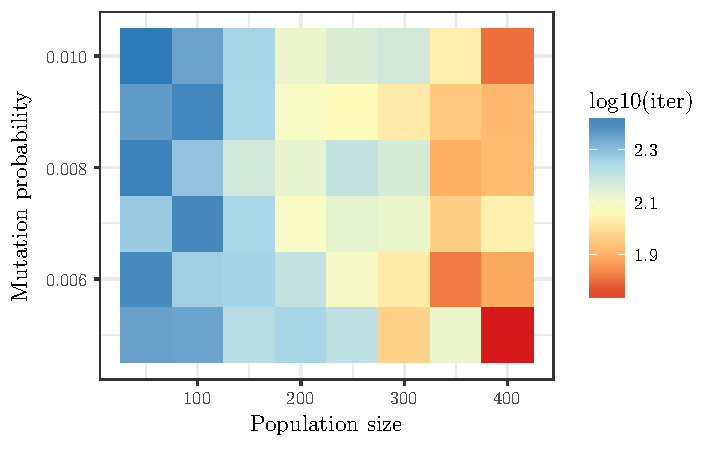
\includegraphics[height=0.5\textwidth]{params_8}
	\caption{Required iterations to find a solution to the $8$ Queens Problem}
	\label{fig:params_8}
\end{figure}

As we can see, it seems the mutation probability $p$ does not play a significant role on the iterations needed to find a solution. To make sure this is really the case, we decided to focus on $N = 8$, and decided to run a more granular version of \cref{sn:bash-script}. The results of these \num{75600} tests can be seen in figure \ref{fig:params_8b}.

\begin{figure}[H]
	\centering
	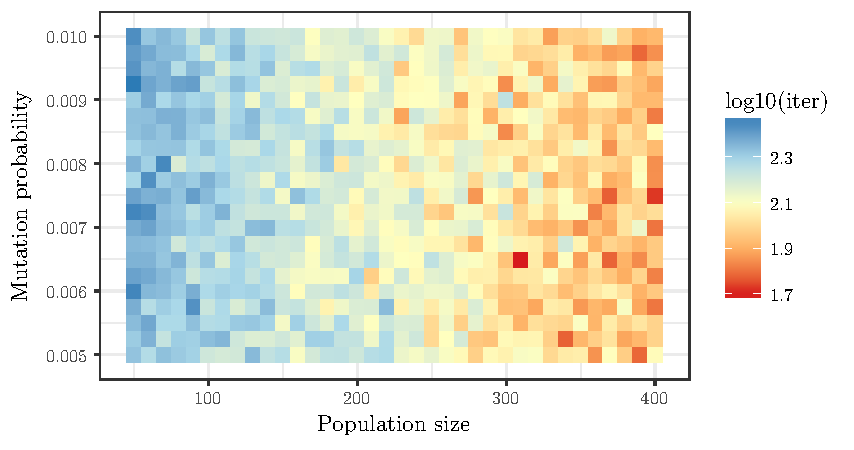
\includegraphics[height=0.5\textwidth]{params_8b}
	\caption{Required iterations to find a solution to the $8$ Queens Problem, using a more granular analysis}
	\label{fig:params_8b}
\end{figure}

Looking at the figure above, our hypothesis seems confirmed. Whilst the dependence on the required iterations with the population size \inline{POPULATION} is more than clear, the mutation probability $p$ seems to be statistically irrelevant on the performance of the Genetic Algorithm.

For this reason, we will retract our previous train of thought and will consider once again the tournament size $\tau$ as variable to be optimised. For the next analysis, we will fix $\inline{POPULATION}$, and play with the following settings:
\begin{itemize}
	\item Mutation: $p \in [0.005, 0.01]$ with a step of $\Delta p = 0.00025$.
	\item Tournament size: $\tau \in [2,7]$ with a step of $\Delta \tau = 1$.
\end{itemize}

In figures \ref{fig:params_8d} and \ref{fig:params_8c} we can see the results of tuning our Genetic Algorithm playing with the mutation probability $p$ and the tournament size $\tau$, with $\inline{POPULATION} = 100, 350$. These two population sizes were chosen to see if we could make an improvement on a slow algorithm ($\inline{POPULATION} = 100$) and a fast one ($\inline{POPULATION} = 350$).

Tuning both parameters do seem to give us a small improvement on the iterations required to find a solution (see table \ref{tab:mins-params}). Yet, it is difficult to say for sure that the results follow a robust pattern; one could argue that there is a sweet-spot for $\tau = 3$, $p \sim 0.009$, debatably the \emph{best configuration of parameters}.

\begin{figure}[H]
	\centering
	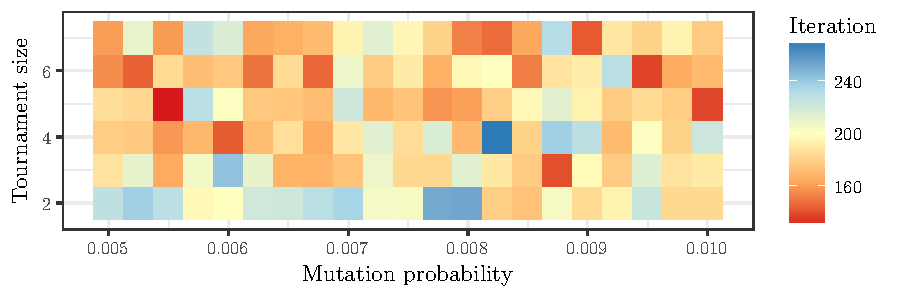
\includegraphics[width=\textwidth]{params_8c}
	\caption{Required iterations to find a solution to the $8$ Queens Problem, with $\inline{POPULATION} = 100$}
	\label{fig:params_8c}
\end{figure}

\begin{figure}[H]
	\centering
	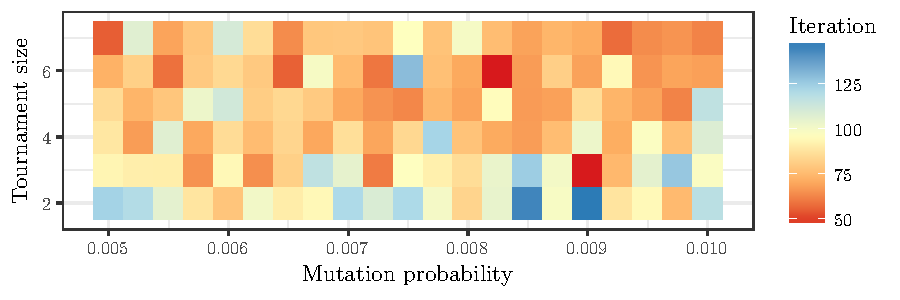
\includegraphics[width=\textwidth]{params_8d}
	\caption{Required iterations to find a solution to the $8$ Queens Problem, with $\inline{POPULATION} = 350$}
	\label{fig:params_8d}
\end{figure}

\begin{table}[H]
	\centering
	\begin{tabular}{r c c}
		\toprule
		\toprule
		\texttt{POPULATION} & 100 & 350 \\
		\midrule
		$\min{f(p)}$        & 150 & 70  \\
		$\min{f(p, \tau)}$  & 130 & 45  \\
		\bottomrule
	\end{tabular}
	\caption{Best mean iteration time to find a solution to the $8$ Queens Problem}
	\label{tab:mins-params}
\end{table}

%-----------------------------------------------------------------
\subsection{Discussion}
% Genetic Algorithms are a really powerful metaheuristic.

Throughout this text and analysis, our approach has always been quite exploratory compared to algorithms implemented with more elitist selection methods, or using $p \leq 1$. The reason being that if we really cared for having a fast-converging algorithm, we could have used better suited algorithms for the $N$ Queens Problem, such as Recursive Backtracking.

After running the algorithm more than \num{115000} times, I can only say \textcite{Michalewicz2000} are unquestionably right; finding a consistently perfect configuration of parameters for a given problem can indeed feel like a hopeless task.

Notwithstanding, this problem and its implementation using a Genetic Algorithm has given us an insightful introduction into the world of metaheuristics, whilst seeing its advantages and limitations.
